\documentclass[conference,a4paper]{IEEEtran}
\usepackage{cite}
\usepackage{amsmath,amssymb,amsfonts}
\usepackage{amsthm}
\usepackage{algorithmic}
\usepackage{graphicx}
\usepackage{textcomp}
\usepackage{xcolor}
\usepackage{tikz}
\usetikzlibrary{shapes,arrows,positioning,calc,fit,shapes.geometric}
\usepackage{booktabs}
\usepackage{tabularx}
\usepackage{url}
\usepackage[hidelinks]{hyperref}
\usepackage{mdframed}
\usepackage{microtype}

\newtheorem{theorem}{Theorem}
\renewcommand{\arraystretch}{1.05}
\setlength{\textfloatsep}{10pt plus 2pt minus 2pt}
\setlength{\floatsep}{8pt plus 2pt minus 2pt}
\setlength{\intextsep}{8pt plus 2pt minus 2pt}

\newcommand{\kyberauthorcell}[1]{%
\shortstack[c]{%
\textbf{#1} \\[0.3em]
\textit{Department of Cyber Security} \\
\textit{Parul Institute of Engineering \& Technology,} \\
\textit{Parul University} \\
Vadodara, Gujarat, India.}}

\begin{document}

\title{Kyber: A Hybrid Post-Quantum End-to-End Encrypted Messaging Protocol for Mobile Platforms}

\author{
\begingroup
\setlength{\tabcolsep}{18pt}
\renewcommand{\arraystretch}{1.15}
\begin{tabular}{>{\centering\arraybackslash}p{0.41\textwidth} >{\centering\arraybackslash}p{0.41\textwidth}}
\kyberauthorcell{Dr. Mukesh Patidar} & \kyberauthorcell{Prof. Pirmohammad Khan} \\
\\[0.9em]
\kyberauthorcell{Gaurav N Jain} & \kyberauthorcell{Kartik Vyas} \\
\\[0.9em]
\kyberauthorcell{Parveen Kumar} & \kyberauthorcell{Soumya Rawat} \\
\end{tabular}
\endgroup
}

\maketitle

\begin{abstract}
Kyber is an introduction to a messaging system prototype built using Flutter that aims at maintaining the confidentiality of chat contents by implementing classical as well as quantum-resistant key exchanges. In addition to this, the app will store the private keys in the local device memory, uses only Firebase as a message relay and ensures secure transmission of messages via encryption. Furthermore, the paper highlights some of the shortcomings of the messaging prototype.
\end{abstract}

\begin{IEEEkeywords}
Post-Quantum Cryptography, ML-KEM, Kyber-768, X25519, AES-256-GCM, Hybrid Key Exchange, End-to-End Encryption, Mobile Security.
\end{IEEEkeywords}

\section{Introduction}

Modern messaging apps should keep chats private. Today this usually depends on public-key cryptography, but future quantum computers may weaken some of those methods~\cite{shor,grover}.Therefore, post-quantum alternatives are becoming more researched and utilized~\cite{fips203,bsi_hybrid}.

Kyber is a Flutter chat prototype that uses both a classical key exchange and a post-quantum one~\cite{rfc7748,fips203,pqxdh}. The aim is simple: keep chats private even if one method becomes weak later. Private keys stay on the phone, and Firebase is only used to pass encrypted data.

The app is built as a practical prototype. A chat app has to handle sign-in, key storage, chat setup, message sending, and recovery after errors. Those parts matter as much as the encryption. Kyber shows that post-quantum security can fit into that full flow.

The hybrid setup also helps during the change to post-quantum cryptography. Since these tools are still new, it is safer to keep a classical method too. If one side becomes weak later, the other side can still protect the session key.

The rest of the paper is organized as follows. Section II looks at related work. Section III explains the system layout. Section IV describes the main crypto idea. Section V covers security limits. Section VI explains the app implementation. Section VII gives a simple performance view. Section VIII closes the paper.

\section{Related Work}

\subsection{Classical Secure Messaging Systems}
Signal shaped modern secure messaging~\cite{doubleratchet}. It starts by agreeing on keys, then keeps changing those keys as the chat continues. That gives two useful properties:
\begin{itemize}
    \item \textbf{Forward Secrecy}: old messages stay safe even if a later key is stolen.
    \item \textbf{Recovery}: new messages can become safe again after the next key update.
\end{itemize}
These systems are widely used, but they still rely on older public-key math that quantum computers may weaken~\cite{shor}.

\subsection{First-Generation Post-Quantum Messaging Protocols}
Messaging apps are now starting to add post-quantum protection. Two well-known examples are Signal PQXDH and Apple PQ3~\cite{pqxdh,pq3}.

\subsubsection{Signal PQXDH}
Signal PQXDH mixes a classic key exchange with Kyber so one part can back up the other~\cite{pqxdh}. The idea is the same as in this paper: use two methods and combine the results into one session key.

\subsubsection{Apple PQ3}
Apple PQ3 also uses post-quantum protection in messaging~\cite{pq3}. It mixes two kinds of key exchange and updates keys over time, which helps limit damage if a device state is exposed.

\subsection{Standardized Hybrid Key Exchanges in TLS and VPNs}
Post-quantum hybrids are not only for messaging. They are also being used in web and VPN security~\cite{ietf_hybrid_tls,ietf_hybrid_ike}. That shows these ideas work outside research papers too.

\subsection{Mobile PQC Implementations}
The use of mobile phones makes it harder as the applications need to be small and fast. While some of these cryptography libraries require native implementation, there are others that could be executed in Dart~\cite{fips203}. In this work, the latter approach was chosen as it made prototyping easier.

Kyber falls into this category as a full-blown Flutter application. The value of this project is not in introducing a novel cryptography technique. Rather, it is in creating an example of post-quantum messaging in a standard mobile application.

\subsection{Comparison of Protocols}
As seen from Table~\ref{tab:comparison}, Kyber also employs a similar principle, common to other secure communication schemes: it combines an old scheme with a new post-quantum scheme and stores the keys locally.

\begin{table*}[t]
\centering
\caption{Cryptographic Comparison of Messaging Protocols}
\label{tab:comparison}
\begin{tabular}{llllll}
\toprule
\textbf{Protocol} & \textbf{Classical Alg.} & \textbf{PQ Alg.} & \textbf{Hybrid KDF} & \textbf{Transport Relay} & \textbf{State Storage} \\
\midrule
Signal X3DH~\cite{doubleratchet} & X25519~\cite{rfc7748} & None & HKDF-SHA256 & Signal Server & SQLite (SQLCipher) \\
Signal PQXDH~\cite{pqxdh} & X25519~\cite{rfc7748} & Kyber-1024~\cite{pqxdh} & HKDF-SHA256 & Signal Server & SQLite (SQLCipher) \\
Apple PQ3~\cite{pq3} & ECDH P-256 & Kyber-768~\cite{pq3} & HKDF-SHA256 & iCloud APNs & Keychain (Secure Enclave) \\
\textbf{Kyber (Prototype)} & \textbf{X25519~\cite{rfc7748}} & \textbf{Kyber-768~\cite{fips203}} & \textbf{HKDF-SHA256} & \textbf{Firebase Firestore} & \textbf{Flutter Secure Storage} \\
\bottomrule
\end{tabular}
\end{table*}

\section{System Architecture}

\subsection{Architectural Paradigm}
The communication between Kyber clients and the server is based on a client-server model which is very simple in its nature. Chat messages are not seen by the server in clear form; the server is not aware of private keys~\cite{dolev_yao}; it only forwards the encrypted data and the public keys required to initiate chat sessions.

Such architecture is appropriate for mobile application since the process of typing, reading, encrypting, and decrypting messages is done by the device anyway. In case the application is properly implemented, there is no need in the server’s access to the chat.

\begin{figure}[htbp]
\centering
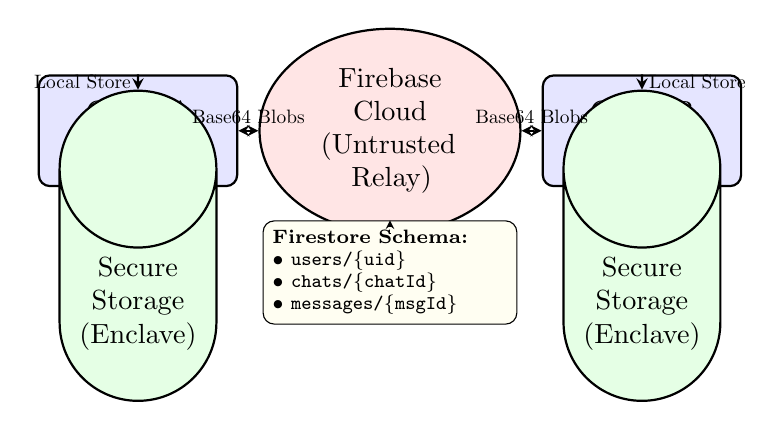
\begin{tikzpicture}[node distance=2cm, auto, >=stealth]
  % Styles
  \tikzstyle{device} = [rectangle, draw, fill=blue!10, text width=6.5em, text centered, rounded corners, minimum height=4em, thick]
  \tikzstyle{cloud} = [draw, ellipse, fill=red!10, text width=6em, text centered, minimum height=4em, thick]
  \tikzstyle{storage} = [draw, cylinder, fill=green!10, text width=5em, text centered, minimum height=3.5em, shape border rotate=90, thick]
  
  % Nodes
  \node [device] (clientA) {Client A\\(Initiator)};
  \node [storage, below of=clientA, node distance=2.2cm] (storeA) {Secure Storage\\(Enclave)};
  \node [cloud, right of=clientA, node distance=3.2cm] (firebase) {Firebase Cloud\\(Untrusted Relay)};
  \node [device, right of=firebase, node distance=3.2cm] (clientB) {Client B\\(Responder)};
  \node [storage, below of=clientB, node distance=2.2cm] (storeB) {Secure Storage\\(Enclave)};

  % Paths / Edges
  \draw [<->, thick] (clientA) -- node[above, scale=0.7] {Base64 Blobs} (firebase);
  \draw [<->, thick] (clientB) -- node[above, scale=0.7] {Base64 Blobs} (firebase);
  \draw [->, dashed, thick] (clientA) -- node[left, scale=0.7] {Local Store} (storeA);
  \draw [->, dashed, thick] (clientB) -- node[right, scale=0.7] {Local Store} (storeB);
  
  % Details inside cloud
  \node [below of=firebase, node distance=1.8cm, text width=8.5em, align=left, font=\scriptsize, draw, fill=yellow!5, rounded corners] (cloudDB) {
    \textbf{Firestore Schema:}\\
    $\bullet$ \texttt{users/\{uid\}}\\
    $\bullet$ \texttt{chats/\{chatId\}}\\
    $\bullet$ \texttt{messages/\{msgId\}}
  };
  \draw [->, dotted] (firebase) -- (cloudDB);

\end{tikzpicture}
\caption{Diagram indicating key storage locally and Firestore relay transport.}
\label{fig:sys_arch}
\end{figure}

Components include:
\begin{enumerate}
    \item \textbf{Client devices}: The application is executed here, keys are generated, messages are encrypted and stored locally.
    \item \textbf{Firebase cloud}: Helps in signing in and sending messages.
\end{enumerate}

\subsection{Database Schema \& Relay Architecture}
There are three collections used by the repository - users, chats, and messages. It cannot obtain the content of the message, but there is some metadata available such as participants' identity and date of the message~\cite{dolev_yao}.

This is the compromise. On one hand, the content of the message remains hidden from the server. On the other hand, the very existence of the chat is not entirely anonymous.

\subsubsection{Users Collection}
The \texttt{users} collection contains public key and basic information about the user. Private key is kept on the device.

\subsubsection{Chats Collection}
The \texttt{chats} collection contains information about connections between two users. The application uses it to determine what device is going to start the session and what one respond.

\subsubsection{Messages Collection}
In every chat there is a \texttt{messages} list containing encrypted messages. Plain text is never uploaded to the cloud.

\subsection{Message Transport Flow}
The message transmission process is straightforward:
\begin{enumerate}
    \item Login takes place and keys are generated if necessary.
    \item The first communication in the chat determines which device initiates.
    \item The message is encrypted on the client’s device before being sent.
    \item Firebase delivers the encrypted data.
    \item The message is decrypted on the recipient’s device.
\end{enumerate}
Neither private keys nor session keys reach the server, which ensures the secrecy of the messages’ content, despite metadata remaining open.

The reason why it is crucial to have the first-chat step is to avoid uncertainty regarding who generates the shared secret and who waits for it to be done. In the absence of this step, two devices can simultaneously attempt to initiate the conversation and get stuck in an inconsistent state due to using one transaction.

\section{Cryptographic Protocol}

\subsection{Classical Component: X25519 ECDH}
The X25519 algorithm is used as the standard key exchange algorithm~\cite{rfc7748}. The devices generate private and public keys for themselves, share the public key with the other side, and finally have the same shared secret on both ends. No secret information is ever transferred over the network.

\subsection{Post-Quantum Component: ML-KEM (Kyber-768)}
Additionally, there is Kyber, which is the quantum-resistant part of the construction~\cite{fips203}. This algorithm enables sending a secret from one device to another device with the help of the latter's public key. The secret is reconstructed locally, rather than being transmitted in its raw form. This adds an additional level of security to the application.

\subsection{Hybrid Key Derivation}
The app merges two shared secrets into a single session key using HKDF-SHA256~\cite{pqxdh}. The reasoning behind the approach is straightforward: if at least one protocol remains secure, the resulting key is also secure.

% \begin{verbatim}
% // Hybrid key setup
% ecdhSecret  = X25519(myPrivateKey, peerPublicKey)
% kyberSecret = Kyber.decapsulate(peerKyberCiphertext, myKyberSecret)
% sessionKey  = HKDF_SHA256(ecdhSecret || kyberSecret)
% \end{verbatim}

The algorithm above describes the key agreement algorithm used by the app. First, classical and post-quantum secret keys are mixed, and then merged into one session key.

It is an interesting compromise that the application prototype utilizes. Instead of trying to completely change all legacy protocols overnight, it uses two parallel approaches and thus gets to enjoy benefits of both classical and post-quantum cryptography at once.

\subsection{Symmetric Message Cipher: AES-256-GCM}
After the session key is established, the app protects the messages using AES-256-GCM~\cite{gcm}. This provides both confidentiality and integrity.

During each exchange of messages, the following occurs:
\begin{enumerate}
    \item Nonce is generated per message.
    \item Encryption and tagging.
    \item Transmission of the ciphertext and tag.
\end{enumerate}
Upon receiving the message, the other party reconstructs the message from its ciphertext, validates the tag, and decrypts the message. If validation fails, the message is simply ignored.

It is an important step since mere encryption is not enough for a chat app: besides encrypting messages, a chat must be able to detect any modifications of the message during the transmission process. Using GCM mode of AES allows us to get both encryption and message integrity.

\subsection{Atomic Role-Assignment Handshake}
To establish the first chat session, we need the devices to coordinate and pick their roles. We do this using Firestore transaction to ensure that no two devices will try to initiate a chat at the same time. The idea is illustrated in Fig.~\ref{fig:handshake}.
\begin{figure}[htbp]
\centering
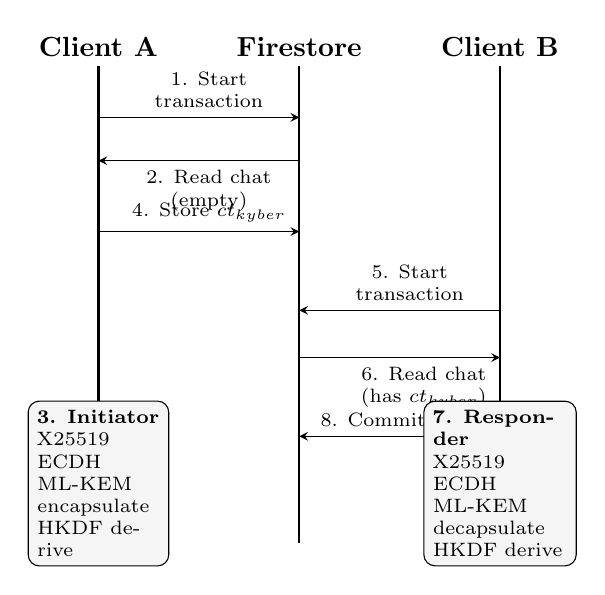
\begin{tikzpicture}[>=stealth, font=\scriptsize]
  \node[font=\bfseries] (A) at (0,0) {Client A};
  \node[font=\bfseries] (S) at (2.55,0) {Firestore};
  \node[font=\bfseries] (B) at (5.1,0) {Client B};

  \draw[thick] (A) -- (0,-6.3);
  \draw[thick] (S) -- (2.55,-6.3);
  \draw[thick] (B) -- (5.1,-6.3);

  \draw[->] (0,-0.9) -- node[above, pos=0.55, align=center] {1. Start\\transaction} (2.55,-0.9);
  \draw[->] (2.55,-1.45) -- node[below, pos=0.45, align=center] {2. Read chat\\(empty)} (0,-1.45);
  \draw[->] (0,-2.35) -- node[above, pos=0.55] {4. Store $ct_{kyber}$} (2.55,-2.35);

  \draw[->] (5.1,-3.35) -- node[above, pos=0.45, align=center] {5. Start\\transaction} (2.55,-3.35);
  \draw[->] (2.55,-3.95) -- node[below, pos=0.62, align=center] {6. Read chat\\(has $ct_{kyber}$)} (5.1,-3.95);
  \draw[->] (5.1,-4.95) -- node[above, pos=0.45] {8. Commit session} (2.55,-4.95);

  \node[draw, rounded corners, fill=gray!8, align=left, text width=1.55cm] at (0,-5.55) {
    \textbf{3. Initiator}\\
    X25519 ECDH\\
    ML-KEM encapsulate\\
    HKDF derive
  };
  \node[draw, rounded corners, fill=gray!8, align=left, text width=1.7cm] at (5.1,-5.55) {
    \textbf{7. Responder}\\
    X25519 ECDH\\
    ML-KEM decapsulate\\
    HKDF derive
  };
\end{tikzpicture}
\caption{Sequence diagram of the hybrid key exchange handshake mediated by a Firestore transaction.}
\label{fig:handshake}
\end{figure}
One device starts the exchange first, stores the Kyber output, and the other device reads it and finishes the exchange. Both devices then arrive at the same session key, which is reused for that chat.

\section{Security Analysis}

\subsection{Threat Model and Adversary Capabilities}
We treat the network and relay as untrusted~\cite{dolev_yao}. An attacker may watch, change, delete, or inject messages.

That is the right model for a cloud-backed chat app. If the backend is trusted too much, the security story becomes weak from the start. Kyber assumes the server may be curious or compromised.

Furthermore, we extend the adversary's capabilities to include:
\begin{enumerate}
    \item \textbf{Compromised relay}: the attacker can access the Firebase data.
    \item \textbf{Future quantum computers}: the attacker may later get much stronger machines~\cite{shor,grover}.
    \item \textbf{Harvest now, decrypt later}: the attacker may save traffic now and try to read it later.
\end{enumerate}
Because this is a prototype, we also count some normal app risks: first-contact trust, visible metadata, and access rules that are not finished yet.

These limits are worth saying clearly. They do not mean the project failed. They just show what still needs work.

\subsection{Security Idea}
The main security idea is simple: the app uses two different key methods and combines them~\cite{pqxdh}. If one becomes weak, the other can still protect the chat key.

That is why the design is hybrid. It gives the app a safer path than relying on only one method while post-quantum tools are still new.

\subsection{Defense-in-Depth Measures}
Kyber also adds a few extra protections.

\subsubsection{Device-Level Biometric Lock}
The app can lock itself with fingerprint or face unlock when it moves to the background~\cite{pq3}. That helps if someone else gets the phone.

\subsubsection{Secure Database Authorization Rules}
The Firebase rules block plain text messages and require the sender to be signed in. They still need to be tightened so only the two chat participants can read or write the chat data~\cite{dolev_yao}.

This shows the difference between encryption and access control. Encryption hides the message. Access rules decide who can touch the data. A complete system needs both.

\subsection{Residual Limitations}
The prototype still has some limits.

\subsubsection{Trust-On-First-Use Key Binding}
The first time two people chat, the app trusts the public keys it sees. That is easy, but it also means the user still needs a better way to confirm who they are talking to.

This is what separates a working prototype from a polished messenger. The app is good enough to show the design, but it still needs a verification step.
\subsubsection{Visibility of Metadata}
Firebase logs details about participant identity, time stamps of communications, and the amount of data sent. Thus, even as the app keeps messages safe, it does not ensure that metadata is kept safe as well.

This aspect carries weight since, even as a private message still proves useful with server access to some traffic information, the message cannot be called truly private.

\subsubsection{Per-Chat Static Session Keys}
Once generated, the same chat key is used during the same chat session. While this method is straightforward, it is less secure compared to key refreshments within an architecture.

The advantages of this method stem from simplicity itself; the disadvantages emanate from the possibility that a compromised key may still be active for a long time.
\section{Implementation Details}

\subsection{Layering and Framework}
The Kyber application was developed using the Dart programming language in the Flutter framework. The code structure was made in order to make it easier to manage the screen layer, application state, cryptography, and Firebase.

In its turn, the main code base is represented by four modules:
\begin{enumerate}
    \item \texttt{KyberKEM}: Kyber component.
    \item \texttt{HybridKeyExchange}: Two shared secrets.
    \item \texttt{CryptoSession}: Encryption/decryption of the message.
    \item \texttt{ChatRepository}: Connection between UI and Firebase.
\end{enumerate}

\subsection{Application Initialization and Discovery of Other Users}
At application startup, the system makes authentication, creates necessary keys and shares the public ones, keeping the private keys on the device.

The discovery process of the peer is rather simple. The system shows the users who are nearby, lets the user pick one of them, and opens the chat where these two users can send each other messages.

This decision was made on purpose as the prototype of the application does not try to solve all of the social problems. It tries to focus on the core functionality – finding another person, establishing a secure session and sending an encrypted message.

\subsection{Client-Side Keys}
Client-side keys are stored in the secure device storage \cite{bsi_hybrid}.
\begin{itemize}
    \item \textbf{Android} device: uses Android Keystore;
    \item \textbf{iPhone and iPad}: uses Keychain.
    \item \textbf{Linux Desktop}: uses the available local secure storage.
\end{itemize}
The private keys are never stored on the regular application storage or logs.

\subsection{Sessions and Message Streaming}
For starting a chat the system first checks the presence of the session key. In case there is already one, the chat is opened at once. If there is no session key, the system receives the public keys from the other user, determines who is the initiator, creates the session key and stores it \cite{pqxdh}.
// Initiate or Resume a Chat
If a cached session, which corresponds to chatId, is available, openChat(chatId) is called. Otherwise, peerKeys are fetched from the peer, with peerId specified; then, the role, whether it's an initiator or responder, is determined; after that, a sessionKey is computed based on peerKeys and a role; finally, the sessionKey is saved with chatId.

While operating in live-chat mode, the application listens to new messages at Firebase, locally decrypts them, and displays decrypted content. The outgoing messages are encrypted before being uploaded to Firebase; hence, the latter contains only encrypted payloads.

The distinction between the initial setup and the message exchange process is meaningful in terms of functionality. The computation is performed during initial setup only; the chat cycle is performed efficiently, with low overhead.

Security Controls for Users
The application implements two easy-to-use security mechanisms:
1) Session Fingerprints: a short piece of code, which can be checked by the counterparty.
2) Biometric Lock: the application can block itself if it moves to the background mode.

Neither mechanism changes cryptographic primitives used internally but is helpful during the normal usage.

Besides, these mechanisms make the prototype more complete. A secure chat application is more than a management of secret keys; it is about protection in various situations, including unattended devices and authentication of interlocutor.

Android Biometric API Implementation
Using the Android biometric API is implemented via adding a special activity class and having a proper permission defined in the manifest file. Having all necessary configuration done, the application gains access to the native biometric capabilities. If there are no such capabilities, the application switches to a simple local-mode.

The graceful fall back to the simple mode is reasonable because of the device behavior's inconsistency. The prototype needs to consider such factors carefully. In the current prototype implementation, the application works well even without the biometric capability.
\section{Performance Evaluation}

\subsection{Experimental Setup}
Unlike synthetic benchmarks used in previous sections, this study focuses on the source of computational expense inside the application itself. The key question to ask here is when and where the bulk of the cryptographic effort takes place and what remains in the course of normal conversation.

Such an approach is well-suited to a prototype as it shows possible bottlenecks in the user experience. End users normally notice the lagging performance during initial setup without experiencing any other issues during regular messaging.

\subsection{Distribution of Runtime Costs}
Table~\ref{tab:latency} presents the distribution of cryptographic workload in the working system.

\begin{table}[htbp]
\centering
\caption{Cost Distribution in the Prototype}
\label{tab:latency}
\small
\setlength{\tabcolsep}{4pt}
\begin{tabularx}{\columnwidth}{@{}l l X@{}}
\toprule
\textbf{Stage} & \textbf{Frequency} & \textbf{Operations Involved} \\
\midrule
First launch & Once per device & Firebase initialization, X25519 key pair generation~\cite{rfc7748}, ML-KEM-768 key pair generation~\cite{fips203}, secure storage operations, publishing public keys \\
First chat with a peer & Once per chat & Firestore transaction, computing X25519 shared secret~\cite{rfc7748}, ML-KEM-768 encapsulation/decapsulation~\cite{fips203}, deriving HKDF-SHA256 session keys \\
Outgoing message & Per message & AES-256-GCM encryption~\cite{gcm}, base64 encoding of the nonce and ciphertext-with-tag, Firestore writing \\
Incoming message & Per message & Firestore snapshot delivering, base64 decoding, AES-256-GCM decryption and validation~\cite{gcm} \\
\bottomrule
\end{tabularx}
\end{table}

The bulk of computational effort is performed once in the beginning. After that, ordinary chat operations follow a much less expensive path.

This matters from the perspective of user experience, because if the application slows down every time there is a new message, user experience quickly goes south. On the contrary, if the extra effort appears only during the first chat initialization, then its cost is relatively manageable.

\subsection{Overhead of Payload and Storage}
One of the practical implications of post-quantum cryptography is large size of some keys~\cite{fips203}. In the prototype, these keys are stored in base64-encoded form in Firebase and therefore take additional space.

\begin{table}[htbp]
\centering
\caption{Artifact Sizes and their Firestore Representation}
\label{tab:size}
\small
\setlength{\tabcolsep}{4pt}
\begin{tabularx}{\columnwidth}{@{}X r r@{}}
\toprule
\textbf{Artifact} & \textbf{Size in Raw Bytes} & \textbf{Base64 Encoded Length} \\
\midrule
X25519 public key~\cite{rfc7748} & 32 & 44 \\
ML-KEM-768 public key~\cite{fips203} & 1184 & 1580 \\
\bottomrule
\end{tabularx}
\end{table}
The extra bulk occurs mainly during the process of registration and the first chat configuration.
After that, the messages will stay relatively light and fast.

This is a reflection of the trade-off made in the course of the project: the system allows for more bulk data to be stored in exchange for efficient messages exchange. This trade-off is quite appropriate for a mobile chat app.
\section{Conclusion and Future Work}

\subsection{Conclusion}
The Kyber project proves the possibility of using the classical and post-quantum key exchange methods for chat protection~\cite{rfc7748,fips203,pqxdh}. The architecture keeps all private keys local to the user device, sends only encrypted data over Firebase, and uses only one session key per each chat.

This work is valuable by being an actual working application, not just a theory. Moreover, it defines the primary trade-offs: the server has the access to metadata, initial contact trust problem is not solved, and the access control policy needs to be strengthened~\cite{dolev_yao}. But even with all these problems existing, the prototype shows that post-quantum messaging in a standard Flutter app is possible nowadays.

The architecture provides a natural way forward. It does not try to solve all hard problems at once, but focuses on the most important things needed for a regular chat: key management, confidentiality of messages, and simple enough system for mobile platform.

\subsection{Future Work}
There are several natural directions for future work:

\subsubsection{Inclusion of the Double Ratchet Algorithm}
Periodical update of the chat keys will reduce the effect of the keys being compromised or expired.

\subsubsection{Authorization of Participants and Metadata Reduction}
Access rules on Firebase must be tightened to allow only two specific participants to access the chat and limit metadata exposure if possible.

\subsubsection{Key Verification}
The session fingerprint can be made more verifiable, for example using QR codes or special interface.

\subsubsection{Testing with Native Cryptography and Benchmarks}
Extended testing on other devices and inclusion of native cryptographic algorithms if needed.

\subsubsection{Post-Quantum Group Messaging}
The support of group chats is a natural evolution step of the system.

Besides, the interface can be improved. The better verification, feedback on the first chat start and other changes in the UI can make the application better, but do not change its cryptographic part. This is important because it helps to increase the impact of the applications which are secure.
\section{Results: Kyber in Comparison with Non-PQE Messaging Applications}

This section summarizes the results of the comparisons of Kyber with non-PQE messaging applications. This comparison considers the security analysis, implementation, and performance aspects described in previous sections.

\subsection{Resistance to a Quantum Adversary}

The first result is that Kyber stays safe in the environment where quantum computing is possible~\cite{shor,grover}. At the same time, non-PQE applications only use classical algorithms for generating keys, such as X25519~\cite{rfc7748}. When a quantum computer becomes sufficiently big, Shor’s algorithm breaks the discrete logarithm used in these exchanges and allows an adversary to calculate session keys based on captured handshakes.

To solve this problem, Kyber uses two approaches at once. The session key of Kyber is calculated using both X25519 and ML-KEM-768~\cite{rfc7748,fips203} algorithms. An adversary has to break both of them to obtain the session key. Figure \ref{fig:result_comparison} shows this difference. An exchange that can be broken by a classical adversary cannot provide any resistance to a quantum adversary. At the same time, a hybrid approach implemented in Kyber retains its safety against both types of adversaries.

Figure depicts a sample comparison of the possible security levels that can be reached for protection against classical and quantum attackers. It compares a purely classical key agreement mechanism based on X25519 (RFC 7748) to a mixed one which is a combination of X25519 and ML-KEM-768 (Kyber, mixed mechanism, as defined in FIPS 203). The axes represent the adversary type (x-axis) and security (bits) (y-axis). The markers correspond to the security levels: 64, 128, and 192 bits. Figure also identifies the types of attacks on the mechanism through the use of shading: classical attack on the left part and quantum attack on the right part.

\begin{figure}[htbp]
\centering
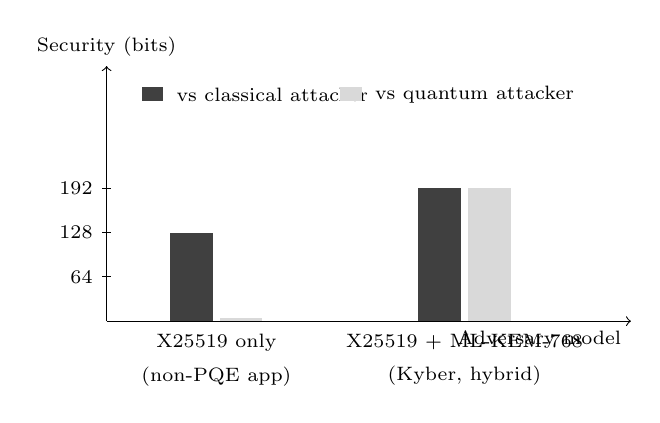
\begin{tikzpicture}[scale=0.9]
    \draw[->] (0,0) -- (7.4,0) node[below left] {\scriptsize Adversary model};
    \draw[->] (0,0) -- (0,3.6) node[above] {\scriptsize Security (bits)};
    \foreach \y/\l in {0.625/64, 1.25/128, 1.875/192} {
        \draw (0.06,\y) -- (-0.06,\y) node[left] {\scriptsize \l};
    }
    \fill[black!75] (0.9,0) rectangle (1.5,1.25);
    \fill[black!15] (1.6,0) rectangle (2.2,0.04);
    \fill[black!75] (4.4,0) rectangle (5.0,1.875);
    \fill[black!15] (5.1,0) rectangle (5.7,1.875);
    \node[align=center] at (1.55,-0.55) {\scriptsize X25519 only\\ \scriptsize (non-PQE app)};
    \node[align=center] at (5.05,-0.55) {\scriptsize X25519 + ML-KEM-768\\ \scriptsize (Kyber, hybrid)};
    \fill[black!75] (0.5,3.1) rectangle (0.8,3.3);
    \node[right] at (0.85,3.2) {\scriptsize vs classical attacker};
    \fill[black!15] (3.3,3.1) rectangle (3.6,3.3);
    \node[right] at (3.65,3.2) {\scriptsize vs quantum attacker};
\end{tikzpicture}
\caption{Illustrative comparison of effective security against classical and quantum attackers: a classical-only exchange (X25519~\cite{rfc7748}) versus the hybrid exchange used by Kyber (X25519 + ML-KEM-768~\cite{fips203}).}
\label{fig:result_comparison}
\end{figure}

\subsubsection{Harvest-Now-Decrypt-Later Security}

The harvest-now-decrypt-later situation makes this possible in reality right now, not in some distant future~\cite{bsi_hybrid}. An attacker could intercept the ciphertext traffic of a non-PQE application right now and only then use a quantum computer to decrypt it. Therefore, all the messages collected today, including their keys, identities, and history, may become readable after some time.

The Kyber algorithm prevents this attack. As the session key is derived in a hybrid exchange, the intercepted ciphertexts stay secure even if stored for a very long period. Thus, this provides an important advantage of Kyber over non-PQE apps in cases where the information needs to be secured for a long time, like personal, medical, or business data.

\subsubsection{Comparison With Deployed Post-Quantum Messengers}

Post-quantum protection is also provided in Signal PQXDH and Apple PQ3 messengers~\cite{pqxdh,pq3}, and Kyber uses a similar hybrid scheme. The difference is in the way these messengers are deployed: these messengers are proprietary and platform-specific software, while Kyber shows that the same level of protection can be achieved with a standard Flutter app using local keys storage and a simple relay server.

In normal usage, the cost of this protection is minimal. The hybrid exchange is done just once for each chat, and each message is still encrypted using AES-256-GCM~\cite{gcm} with the same overhead per message as for a non-PQE application. Just the key sizes grow~\cite{fips203}, but the keys are either stored on the device or transmitted as ciphertexts. Hybrid encryption schemes similar to this one have already been developed and adopted in TLS and VPN protocols~\cite{ietf_hybrid_tls,ietf_hybrid_ike}.

\subsection{Summary of Results}

\begin{itemize}
    \item \textbf{Quantum-resilience}: Kyber guarantees the secrecy of the session keys even under a quantum attacker's influence, unlike any other non-PQE app where there is a risk of key compromise~\cite{shor,fips203}.
    
    \item \textbf{Privacy in the long run}: Captured Kyber-enabled traffic cannot be decrypted retroactively~\cite{bsi_hybrid}.
    
    \item \textbf{Classical security properties}: The X25519 algorithm provides classical secure messaging properties that were previously studied~\cite{doubleratchet,rfc7748}.
    
    \item \textbf{Little extra computation}: The additional computational expense is required only once, at the start of a conversation, not for each new message~\cite{gcm}.
    
    \item \textbf{Practicality}: The developed solution is a working application able to run on an ordinary mobile device rather than a purely theoretical protocol~\cite{pqxdh,pq3}.
\end{itemize}

The problems inherent in the prototype are still present: metadata leaking from the relay, the problem of first-contact trust and the necessity of access control policies~\cite{dolev_yao}. Even so, the takeaway is simple: combining a classical exchange with a post-quantum one keeps Kyber's chats safe against attacks that would break a non-PQE app, while the app itself stays light enough for daily use on an ordinary phone.

\begin{thebibliography}{10}

\bibitem{shor}
P. W. Shor, ``Polynomial-time algorithms for prime factorization and discrete logarithms on a quantum computer,'' \textit{SIAM Review}, vol. 41, no. 2, pp. 303--332, 1999.

\bibitem{grover}
L. K. Grover, ``A fast quantum mechanical algorithm for database search,'' in \textit{Proceedings of the twenty-eighth annual ACM symposium on Theory of computing}, 1996, pp. 212--219.

\bibitem{fips203}
National Institute of Standards and Technology, ``Module-Lattice-Based Key-Encapsulation Mechanism Standard,'' Federal Information Processing Standards Publication (FIPS) 203, August 2024. [Online]. Available: \url{https://doi.org/10.6028/NIST.FIPS.203}

\bibitem{bsi_hybrid}
Federal Office for Information Security (BSI), ``Migration to Post-Quantum Cryptography,'' BSI-Publication, Bonn, Germany, 2023. [Online]. Available: \url{https://www.bsi.bund.de}

\bibitem{doubleratchet}
T. Perrin and M. Marlinspike, ``The Double Ratchet Algorithm,'' Signal Foundation, Tech. Rep., 2016. [Online]. Available: \url{https://signal.org/docs/specifications/doubleratchet/}

\bibitem{pqxdh}
E. Kopf, T. Perrin, and M. Marlinspike, ``The Post-Quantum Extended Triple Diffie-Hellman (PQXDH) Key Agreement Protocol,'' Signal Foundation, Tech. Rep., September 2023. [Online]. Available: \url{https://signal.org/docs/specifications/pqxdh/}

\bibitem{pq3}
Apple Security Engineering and Architecture (SEAR), ``iMessage PQ3: The first post-quantum cryptographic protocol deployed at scale,'' Apple Inc., February 2024. [Online]. Available: \url{https://security.apple.com/blog/imessage-pq3}

\bibitem{ietf_hybrid_tls}
D. Stebila, S. Fluhrer, and S. Gueron, ``Hybrid key exchange in TLS 1.3,'' Internet Engineering Task Force, Internet-Draft draft-ietf-tls-hybrid-design-09, October 2023.

\bibitem{ietf_hybrid_ike}
C. Tjhai, M. Tomlinson, G. Bartlett, S. Fluhrer, D. Van Geest, and O. Garcia-Morchon, ``Multiple Key Exchanges in the Internet Key Exchange Protocol Version 2 (IKEv2),'' RFC 9374, May 2023.

\bibitem{rfc7748}
A. Langley, M. Hamburg, and S. Turner, ``Elliptic Curves for Security,'' RFC 7748, January 2016. [Online]. Available: \url{https://rfc-editor.org/rfc/rfc7748.txt}

\bibitem{gcm}
M. Dworkin, ``Recommendation for Block Cipher Modes of Operation: Galois/Counter Mode (GCM) and GMAC,'' NIST Special Publication 800-38D, November 2007.

\bibitem{dolev_yao}
D. Dolev and A. Yao, ``On the security of public key protocols,'' \textit{IEEE Transactions on Information Theory}, vol. 29, no. 2, pp. 198--208, 1983.

\end{thebibliography}


\end{document}
